%methods 
To accomplish the objective of recolouring the skin tone of a hand to a target colour, we wrote algorithms in C++ in Eclipse on OS X using OpenCV libraries. Eclipse is used to compile each iteration of the algorithm into a debug-mode executable program named Recolor. For ease of testing, as the algorithm is modified, we add more functionality to the Recolor program and retain the ability to use previous versions of the algorithm. We use a custom Python script to run new versions of Recolor from the terminal to test it. All of the relevant code and its versions are hosted on a git repository at github.com/tiantianhan/recolor

Recolor takes as input a hand image, a mask instructing it where to find the average skin colour of the hand, and a desired target skin colour. (Other flags and inputs are also used for testing purposes, see the Github repository readme file for a full description of the usage.) Recolor then outputs the processed image where the skin tone is adjusted to the target colour.

We iterated from simple to more complex algorithms, at each step testing the algorithm and evaluating the results. We tested progressive iterations on a set of hand images with varying skin tones. The images are are shown in Figure \ref{img:input_hands_1}.

%all images that are not test results will be copied to the images folder

\begin{figure}[H]
    \centering
    \begin{subfigure}[b]{0.20\textwidth}
        \includegraphics[width=\textwidth]{images/hand_dark}
        \caption{}\label{img:input_hands_1_dark}
    \end{subfigure}
    ~
    \begin{subfigure}[b]{0.20\textwidth}
        \includegraphics[width=\textwidth]{images/hand_brown}
        \caption{}\label{img:input_hands_1_brown}
    \end{subfigure}
    ~
    \begin{subfigure}[b]{0.20\textwidth}
        \includegraphics[width=\textwidth]{images/hand_light}
        \caption{}\label{img:input_hands_1_light}
    \end{subfigure}
    ~
    \begin{subfigure}[b]{0.20\textwidth}
        \includegraphics[width=\textwidth]{images/hand_pale}
        \caption{}\label{img:input_hands_1_pale}
    \end{subfigure}
    \caption{Different hand images used for testing}\label{img:input_hands_1}
\end{figure}

 For each test, we called the Recolor program to transform the image of one hand to have the skin tone of the hand in another image, then visually compared the processed image to the image of the target hand. We performed the process on all possible combinations of our test images, paying particular attention to the extreme cases, such as transforming from Figure \ref{img:input_hands_1_dark} to Figure \ref{img:input_hands_1_pale} and vice versa, as well as cases that start with a hand with mid-tone skin such as in Figure \ref{img:input_hands_1_brown} (as this is the most likely use case for applications that change the image of a model's hand to match a range of skin tones). We evaluated the resulting images subjectively, based on whether the processed hand looks believably like a hand naturally of that skin tone, and noted any flaws that we then attempted to correct with the next iteration of the algorithm.

In the following subsections we summarize the results of each algorithm and our evaluation of the results.

\subsection{Naive approach: simple addition}
%boost algo
\subsubsection*{Algorithm}
To begin, we performed a simple addition of a value to each of the $RGB$ channels of the hand, such that the average colour of the hand in the processed image is equal to the average colour of the hand in the target image.

% \begin{equation} \label{eq:boost_algo}
% r' = r + \delta_r
% \end{equation}

% Where 

% \begin{equation*}
% \delta_r = \mean{r_t} - \mean{r}
% \end{equation*}

\begin{algorithm}[H]
\caption{Simple addition to $RGB$ channel.}
\label{eq:boost_algo}
\begin{algorithmic}
\State $T$ is the set of pixels in the target image, and $U
\State $\mean{C_T} \gets \Call{Mean}{\vect{C_T}(U)}$
\State $\mean{C_S} \gets \Call{Mean}{\vect{C_S}(V)}$
\For{each pixel $i$}
\State $\vect{C_O}(i) = \vect{C_S}(i) + (\mean{C_{T,U}} - \mean{C_{S,V}})$
\EndFor
\end{algorithmic}
\end{algorithm}

% \nomenclature{$r$}{Value of the red channel of a pixel in the original hand image.}
% \nomenclature{$r'$}{Value of the red channel of the pixel after an algorithm is applied.}
% \nomenclature{$\mean{r}$}{Average value of the red channel of the original hand image.}
% \nomenclature{$\mean{r_t}$}{Average value of the red channel of the target hand image.}
% \nomenclature{$g$}{Value of the green channel of a pixel in the original hand image.}
% \nomenclature{$b$}{Value of the blue channel of a pixel in the original hand image.}

% With the same equation applying for the $g$ and $b$ channels.
\nomenclature{$S$}{The set of pixels in source image.}
\nomenclature{$T$}{The set of pixels in target image.}
\nomenclature{$O$}{The set of pixels in output image.}
\nomenclature{$\mean{C_T, U}$}{The average RGB color of the target hand calculated over region $U$}

\subsubsection*{Results}
In Table \ref{tab:boost_test} we show the results for colour transfers between all possible combinations of our test images.
\begin{longtable}{|N||c|c|c|}
	\caption{Test results of simple addition / subtraction brightening function.\label{tab:boost_test}}\\
	\hline
	\multicolumn{1}{|c||}{No.} & Original & Target & Results \\ 
	\hline
	    \label{row:boost_test_1} &
  \begin{minipage}{.29\textwidth}
    \includegraphics[width=\textwidth,height=\textheight,keepaspectratio]{../inputs/hand_dark.jpg}
  \end{minipage} & 
  \begin{minipage}{.29\textwidth}
    \includegraphics[width=\textwidth,height=\textheight,keepaspectratio]{../inputs/hand_pale.jpg}
  \end{minipage} & 
  \begin{minipage}{.29\textwidth}
    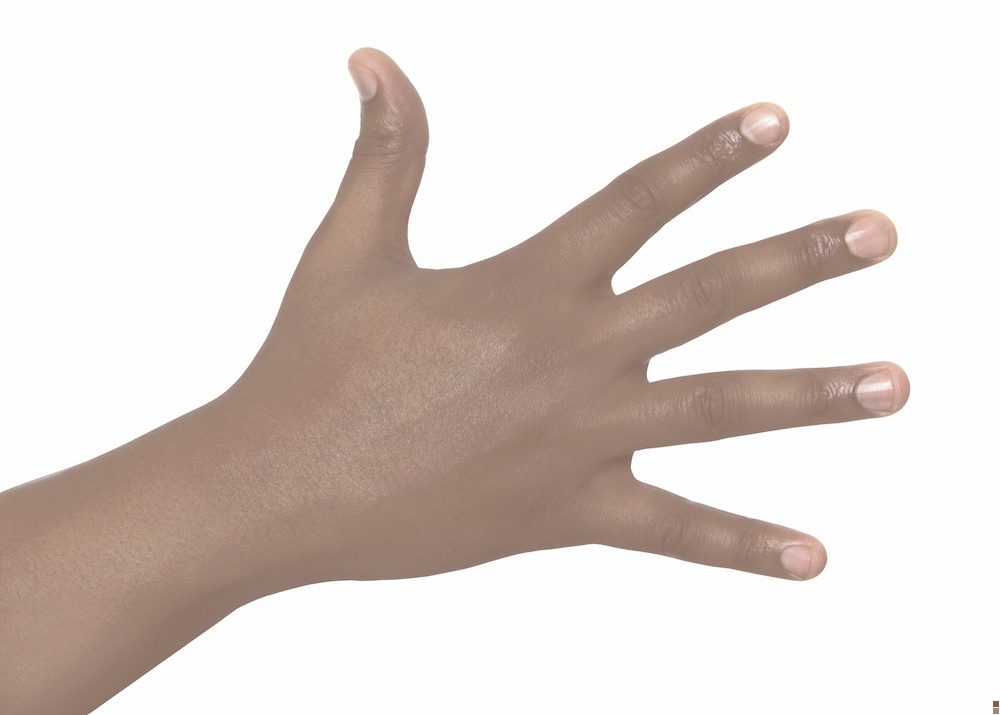
\includegraphics[width=\textwidth,height=\textheight,keepaspectratio]{../rc_test/outputs/debug/hand_dark_to_hand_pale.jpg}
  \end{minipage} \\
\hline
 \end{longtable}

\subsubsection*{Evaluation}
Images of darker skin tones and smaller changes from the original skin tone to the target colour to begin with (Row \ref{row:boost_test_hand_brown_to_hand_dark}) tend to have better results than images with large changes (Rows \ref{row:boost_test_hand_dark_to_hand_light}, \ref{row:boost_test_hand_brown_to_hand_pale}). In the case of changes towards brighter colours, this is because large changes force bright points in the original image to be truncated at white, and also causes dark regions on the image, such as shadows and grooves, to become significantly brighter and less close to true black, giving the image a ``high-key" appearance (Row \ref{row:boost_test_hand_dark_to_hand_light} and \ref{row:boost_test_hand_brown_to_hand_light}).

In addition, we noted that at this stage the transformation from a dark coloured hand to a very pale hand, or even from a mid-toned hand to a pale hand and vice versa is especially unconvincing. (Row \ref{row:boost_test_hand_brown_to_hand_pale}, also see \ref{row:boost_test_hand_dark_to_hand_pale} and \ref{row:boost_test_hand_pale_to_hand_dark})


\subsection{Proportional adjustment relative to average color} \label{sec:algo_prop_eval}
%prop algorithm methods
To correct for the effect of the bright spots in the image being over bright and the high-key appearance resulting from all the shadows being brightened, we used an algorithm that maps the black and white points of the image to the same value, and adjusts the colours in between to match the target average colour.

\begin{algorithm}[H]
\caption{Proportional adjustment relative to average color}
\label{eq:prop_algo}
\begin{algorithmic}
\State $\mean{C_T} \gets \Call{Mean}{\vect{C_T}(U)}$
\State $\mean{C_S} \gets \Call{Mean}{\vect{C_S}(V)}$
\For{each pixel $i \in S$}
\If{$\vect{C_S}(i) \leq \mean{C_S}$}
\State $\vect{C_O}(i) \gets \displaystyle \left(\frac{\mean{C_T}}{\mean{C_S}}\right)\vect{C_S}(i)$
\Else
\State $\vect{C_O}(i) \gets \displaystyle 255 - \left(\frac{255 - \mean{C_T}}{255 - \mean{C_S}}\right)(255 - \vect{C_S}(i))$
\EndIf
\EndFor
\end{algorithmic}
\end{algorithm}

In Table \ref{tab:prop_test} we show the results for colour transfers between all possible combinations of our test images.
\begin{longtable}{|N||c|c|c|}
	\caption{Test results of brightening proportionally based on distance of color to the average.\label{tab:prop_test}}\\
	\hline
	\multicolumn{1}{|c||}{No.} & Original & Target & Results \\ 
	\hline
	    \label{row:prop_test_1} &
  \begin{minipage}{.29\textwidth}
    \includegraphics[width=\textwidth,height=\textheight,keepaspectratio]{../inputs/hand_dark.jpg}
  \end{minipage} & 
  \begin{minipage}{.29\textwidth}
    \includegraphics[width=\textwidth,height=\textheight,keepaspectratio]{../inputs/hand_brown.jpg}
  \end{minipage} & 
  \begin{minipage}{.29\textwidth}
    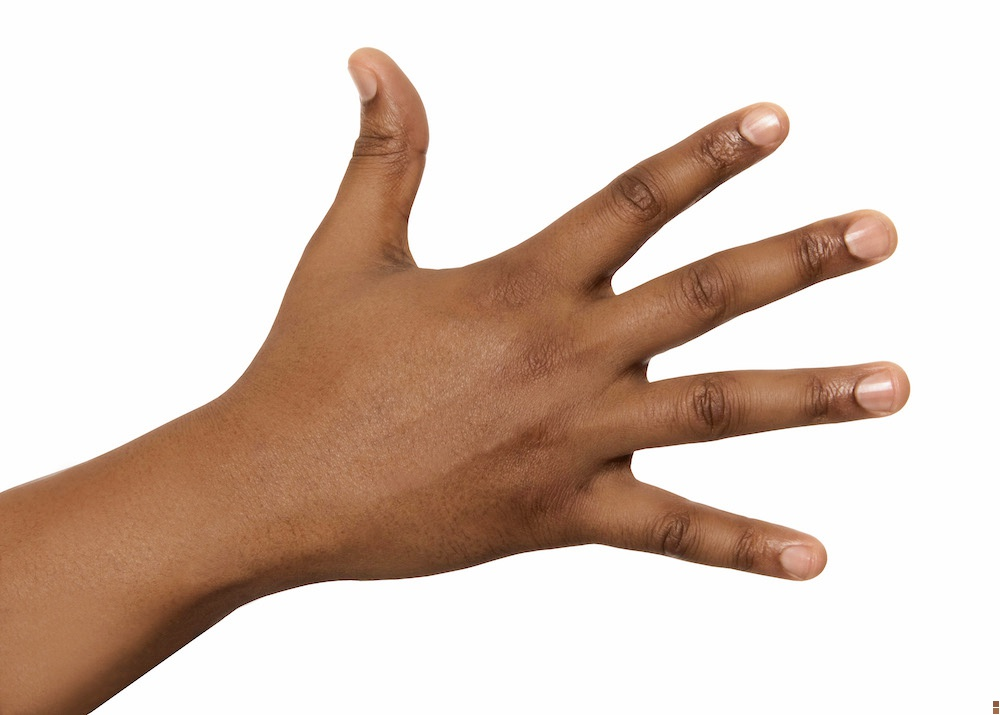
\includegraphics[width=\textwidth,height=\textheight,keepaspectratio]{../rc_test/outputs/20170516_proportional_test/hand_dark_to_hand_brown.jpg}
  \end{minipage} \\
\hline  \label{row:prop_test_1} &
  \begin{minipage}{.29\textwidth}
    \includegraphics[width=\textwidth,height=\textheight,keepaspectratio]{../inputs/hand_dark.jpg}
  \end{minipage} & 
  \begin{minipage}{.29\textwidth}
    \includegraphics[width=\textwidth,height=\textheight,keepaspectratio]{../inputs/hand_light.jpg}
  \end{minipage} & 
  \begin{minipage}{.29\textwidth}
    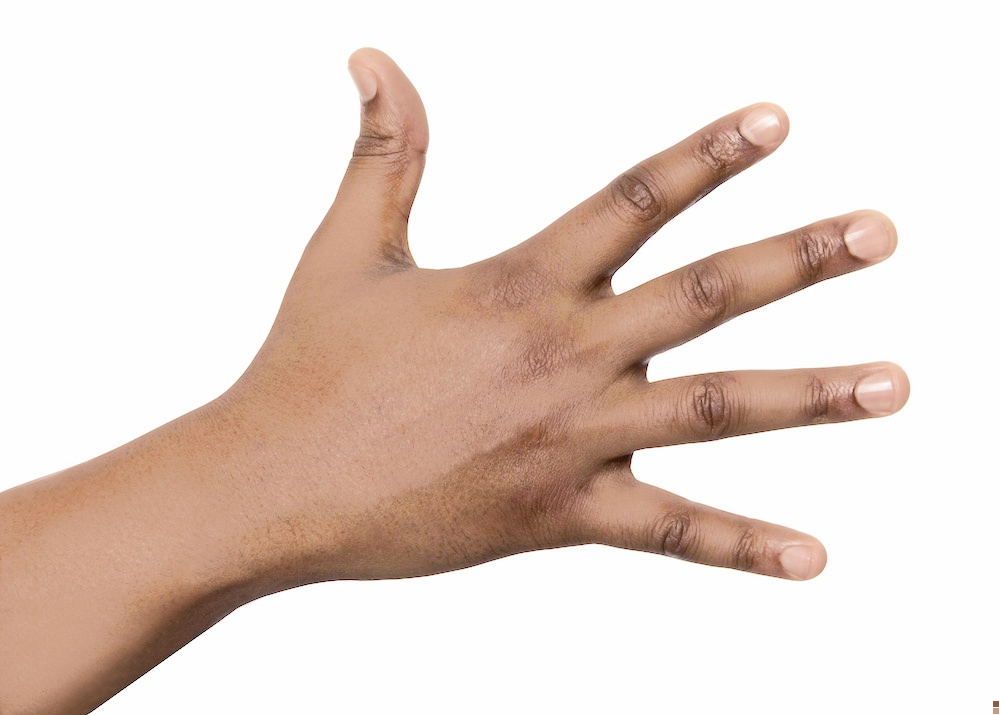
\includegraphics[width=\textwidth,height=\textheight,keepaspectratio]{../rc_test/outputs/20170516_proportional_test/hand_dark_to_hand_light.jpg}
  \end{minipage} \\
\hline  \label{row:prop_test_1} &
  \begin{minipage}{.29\textwidth}
    \includegraphics[width=\textwidth,height=\textheight,keepaspectratio]{../inputs/hand_dark.jpg}
  \end{minipage} & 
  \begin{minipage}{.29\textwidth}
    \includegraphics[width=\textwidth,height=\textheight,keepaspectratio]{../inputs/hand_pale.jpg}
  \end{minipage} & 
  \begin{minipage}{.29\textwidth}
    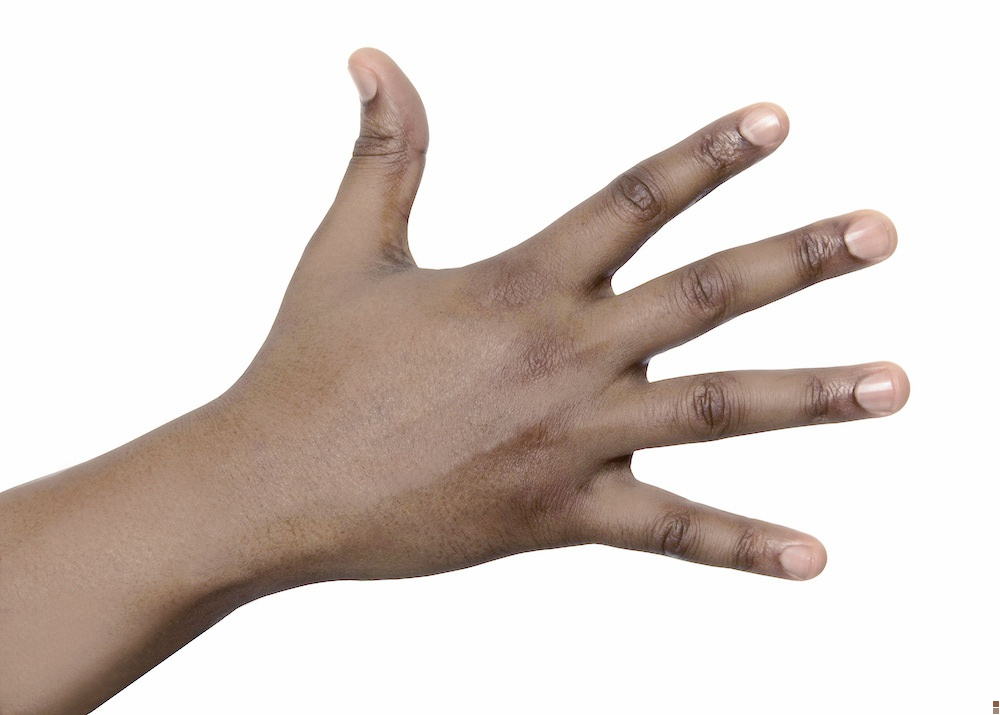
\includegraphics[width=\textwidth,height=\textheight,keepaspectratio]{../rc_test/outputs/20170516_proportional_test/hand_dark_to_hand_pale.jpg}
  \end{minipage} \\
\hline  \label{row:prop_test_1} &
  \begin{minipage}{.29\textwidth}
    \includegraphics[width=\textwidth,height=\textheight,keepaspectratio]{../inputs/hand_brown.jpg}
  \end{minipage} & 
  \begin{minipage}{.29\textwidth}
    \includegraphics[width=\textwidth,height=\textheight,keepaspectratio]{../inputs/hand_dark.jpg}
  \end{minipage} & 
  \begin{minipage}{.29\textwidth}
    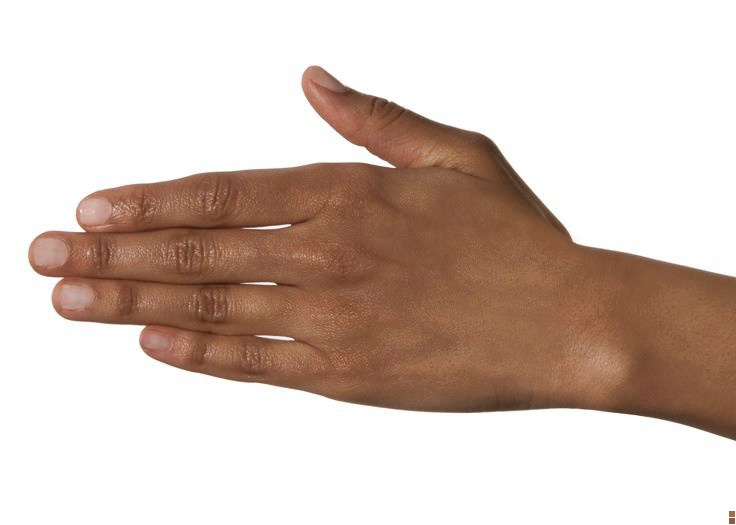
\includegraphics[width=\textwidth,height=\textheight,keepaspectratio]{../rc_test/outputs/20170516_proportional_test/hand_brown_to_hand_dark.jpg}
  \end{minipage} \\
\hline  \label{row:prop_test_1} &
  \begin{minipage}{.29\textwidth}
    \includegraphics[width=\textwidth,height=\textheight,keepaspectratio]{../inputs/hand_brown.jpg}
  \end{minipage} & 
  \begin{minipage}{.29\textwidth}
    \includegraphics[width=\textwidth,height=\textheight,keepaspectratio]{../inputs/hand_light.jpg}
  \end{minipage} & 
  \begin{minipage}{.29\textwidth}
    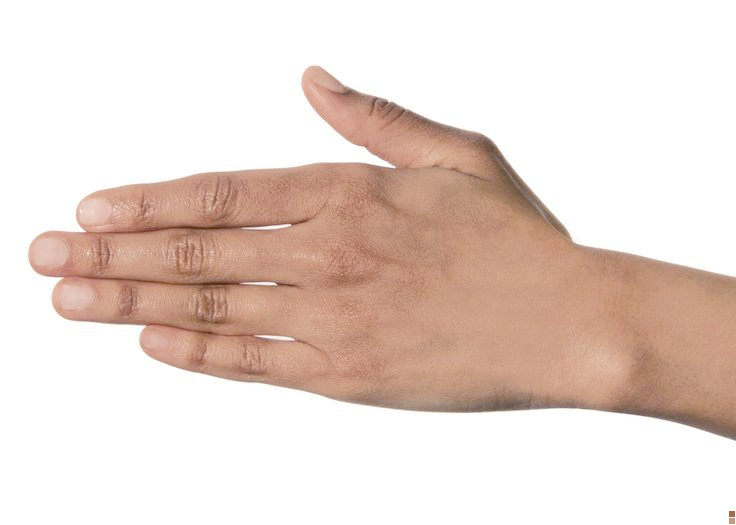
\includegraphics[width=\textwidth,height=\textheight,keepaspectratio]{../rc_test/outputs/20170516_proportional_test/hand_brown_to_hand_light.jpg}
  \end{minipage} \\
\hline  \label{row:prop_test_1} &
  \begin{minipage}{.29\textwidth}
    \includegraphics[width=\textwidth,height=\textheight,keepaspectratio]{../inputs/hand_brown.jpg}
  \end{minipage} & 
  \begin{minipage}{.29\textwidth}
    \includegraphics[width=\textwidth,height=\textheight,keepaspectratio]{../inputs/hand_pale.jpg}
  \end{minipage} & 
  \begin{minipage}{.29\textwidth}
    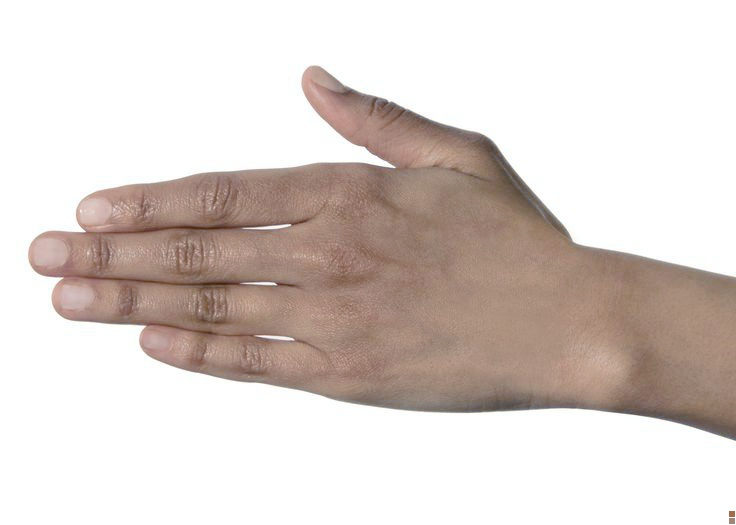
\includegraphics[width=\textwidth,height=\textheight,keepaspectratio]{../rc_test/outputs/20170516_proportional_test/hand_brown_to_hand_pale.jpg}
  \end{minipage} \\
\hline  \label{row:prop_test_1} &
  \begin{minipage}{.29\textwidth}
    \includegraphics[width=\textwidth,height=\textheight,keepaspectratio]{../inputs/hand_light.jpg}
  \end{minipage} & 
  \begin{minipage}{.29\textwidth}
    \includegraphics[width=\textwidth,height=\textheight,keepaspectratio]{../inputs/hand_dark.jpg}
  \end{minipage} & 
  \begin{minipage}{.29\textwidth}
    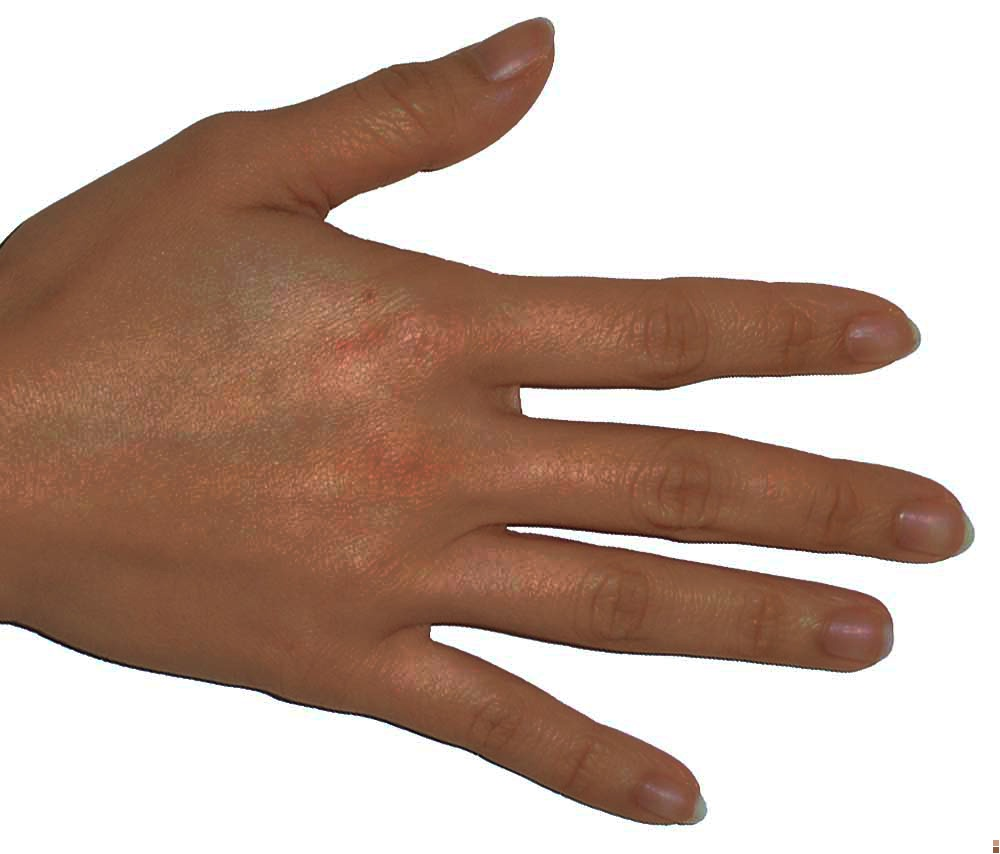
\includegraphics[width=\textwidth,height=\textheight,keepaspectratio]{../rc_test/outputs/20170516_proportional_test/hand_light_to_hand_dark.jpg}
  \end{minipage} \\
\hline  \label{row:prop_test_1} &
  \begin{minipage}{.29\textwidth}
    \includegraphics[width=\textwidth,height=\textheight,keepaspectratio]{../inputs/hand_light.jpg}
  \end{minipage} & 
  \begin{minipage}{.29\textwidth}
    \includegraphics[width=\textwidth,height=\textheight,keepaspectratio]{../inputs/hand_brown.jpg}
  \end{minipage} & 
  \begin{minipage}{.29\textwidth}
    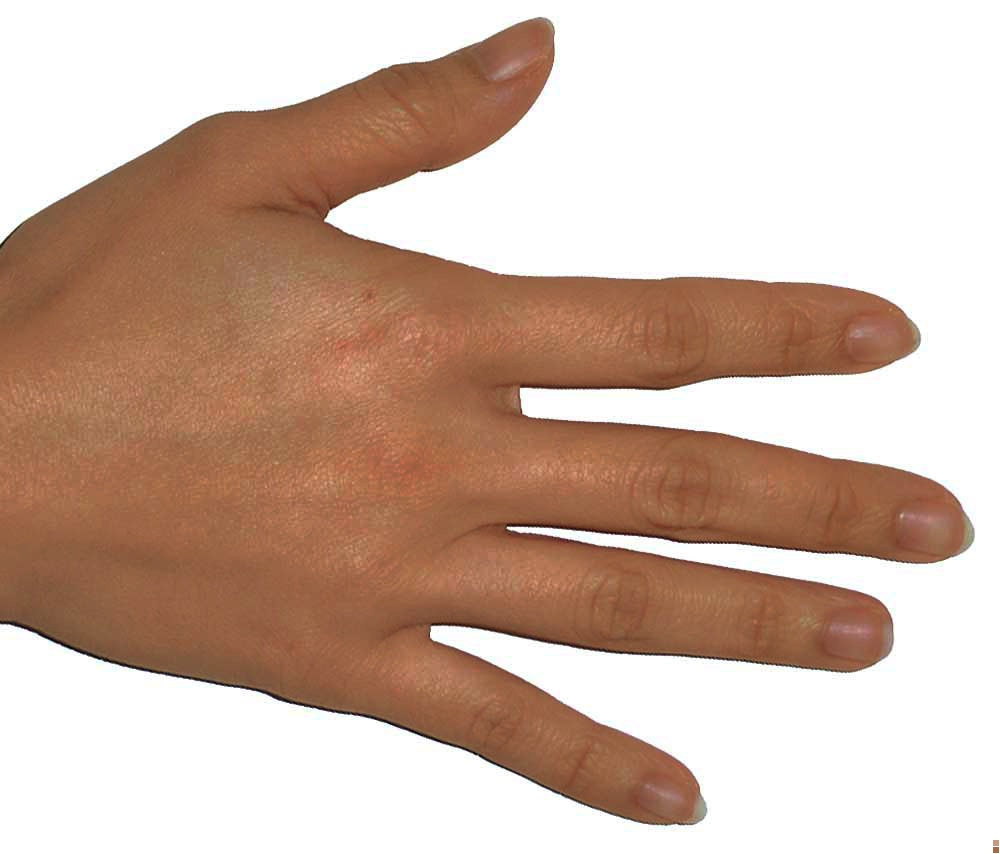
\includegraphics[width=\textwidth,height=\textheight,keepaspectratio]{../rc_test/outputs/20170516_proportional_test/hand_light_to_hand_brown.jpg}
  \end{minipage} \\
\hline  \label{row:prop_test_1} &
  \begin{minipage}{.29\textwidth}
    \includegraphics[width=\textwidth,height=\textheight,keepaspectratio]{../inputs/hand_light.jpg}
  \end{minipage} & 
  \begin{minipage}{.29\textwidth}
    \includegraphics[width=\textwidth,height=\textheight,keepaspectratio]{../inputs/hand_pale.jpg}
  \end{minipage} & 
  \begin{minipage}{.29\textwidth}
    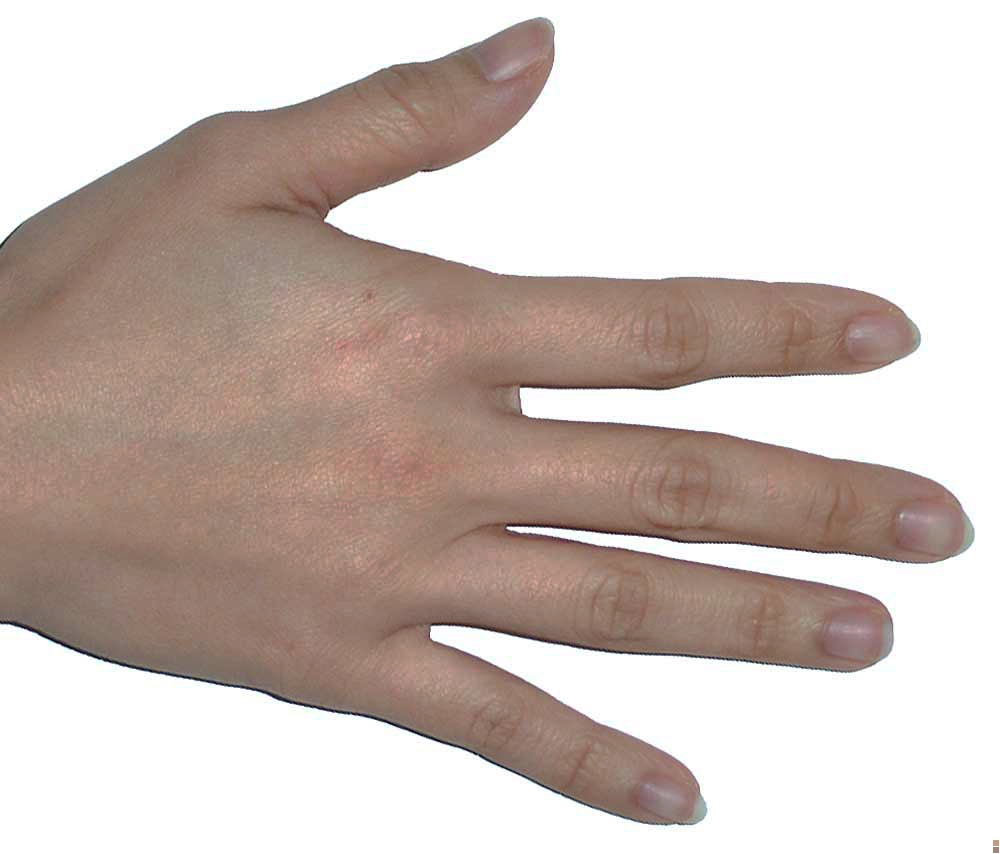
\includegraphics[width=\textwidth,height=\textheight,keepaspectratio]{../rc_test/outputs/20170516_proportional_test/hand_light_to_hand_pale.jpg}
  \end{minipage} \\
\hline  \label{row:prop_test_1} &
  \begin{minipage}{.29\textwidth}
    \includegraphics[width=\textwidth,height=\textheight,keepaspectratio]{../inputs/hand_pale.jpg}
  \end{minipage} & 
  \begin{minipage}{.29\textwidth}
    \includegraphics[width=\textwidth,height=\textheight,keepaspectratio]{../inputs/hand_dark.jpg}
  \end{minipage} & 
  \begin{minipage}{.29\textwidth}
    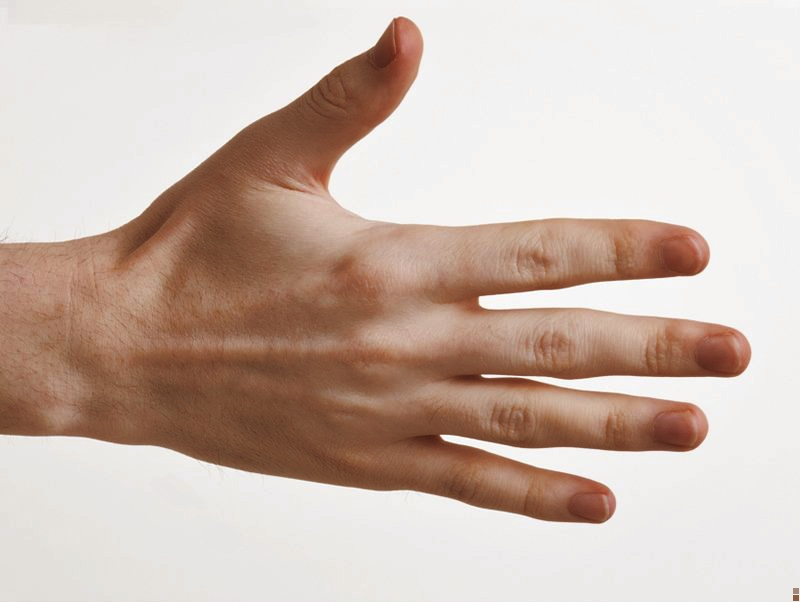
\includegraphics[width=\textwidth,height=\textheight,keepaspectratio]{../rc_test/outputs/20170516_proportional_test/hand_pale_to_hand_dark.jpg}
  \end{minipage} \\
\hline  \label{row:prop_test_1} &
  \begin{minipage}{.29\textwidth}
    \includegraphics[width=\textwidth,height=\textheight,keepaspectratio]{../inputs/hand_pale.jpg}
  \end{minipage} & 
  \begin{minipage}{.29\textwidth}
    \includegraphics[width=\textwidth,height=\textheight,keepaspectratio]{../inputs/hand_brown.jpg}
  \end{minipage} & 
  \begin{minipage}{.29\textwidth}
    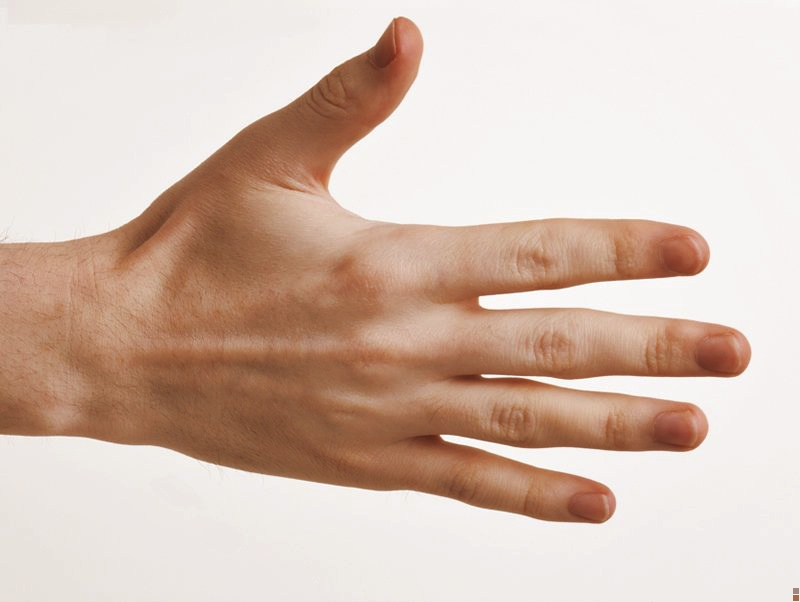
\includegraphics[width=\textwidth,height=\textheight,keepaspectratio]{../rc_test/outputs/20170516_proportional_test/hand_pale_to_hand_brown.jpg}
  \end{minipage} \\
\hline  \label{row:prop_test_1} &
  \begin{minipage}{.29\textwidth}
    \includegraphics[width=\textwidth,height=\textheight,keepaspectratio]{../inputs/hand_pale.jpg}
  \end{minipage} & 
  \begin{minipage}{.29\textwidth}
    \includegraphics[width=\textwidth,height=\textheight,keepaspectratio]{../inputs/hand_light.jpg}
  \end{minipage} & 
  \begin{minipage}{.29\textwidth}
    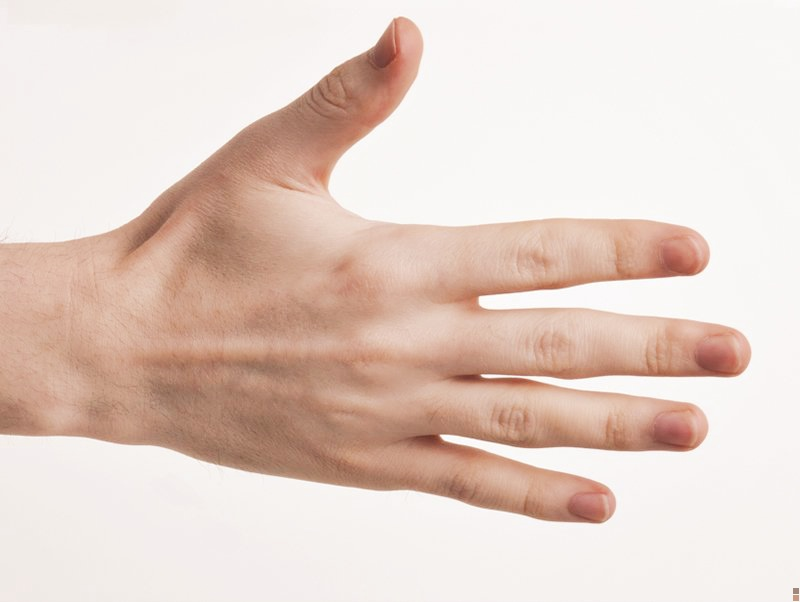
\includegraphics[width=\textwidth,height=\textheight,keepaspectratio]{../rc_test/outputs/20170516_proportional_test/hand_pale_to_hand_light.jpg}
  \end{minipage} \\
\hline
 \end{longtable}

This method improved the appearance of cases with over-bright spots or ``high-key" appearance issues, as Figure \ref{img:compare_bright_spot} shows:
\begin{figure}[H]
    \centering
    \begin{subfigure}[b]{0.40\textwidth}
        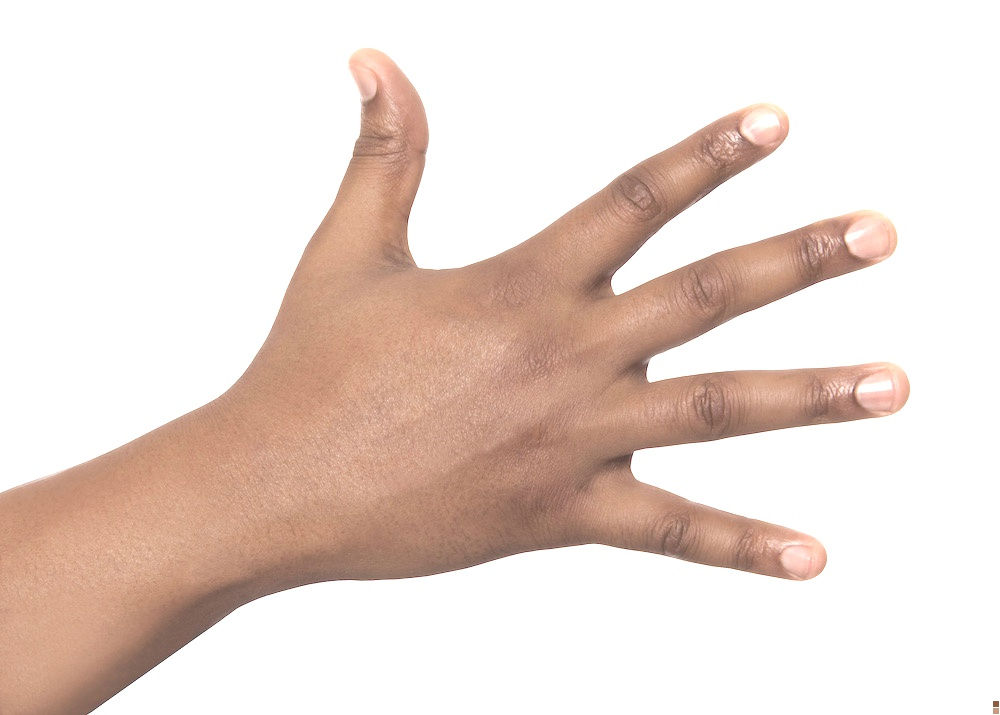
\includegraphics[width=\textwidth]{../rc_test/outputs/20170516_boost_test/hand_dark_to_hand_light.jpg}
        \caption{Simple addition algorithm (Equation \ref{eq:boost_algo})result}
    \end{subfigure}
    ~
    \begin{subfigure}[b]{0.40\textwidth}
        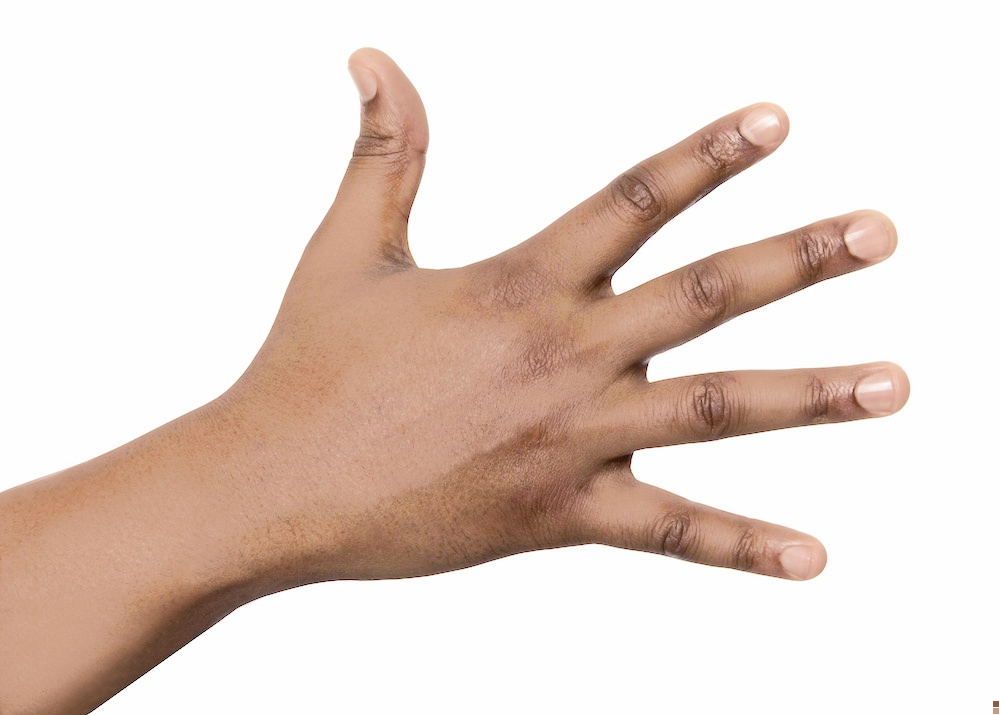
\includegraphics[width=\textwidth]{../rc_test/outputs/20170516_proportional_test/hand_dark_to_hand_light.jpg}
        \caption{Proportional adjustment algorithm (Equation \ref{eq:prop_algo}) result}
    \end{subfigure}
    \caption{Comparison of algorithms \ref{eq:boost_algo} and \ref{eq:prop_algo} results for transforming a dark hand (Figure \ref{img:input_hands_1_dark}) to a light hand (Figure \ref{img:input_hands_1_light}).\label{img:compare_bright_spot}}
\end{figure}

We noted however, that this method noticeably does not correct for, and even exacerbates slightly relative to the simple addition algorithm the dark spots at the joints and creases of a hand of darker skin tone when it is transformed to a lighter skin tone (Row \ref{row:prop_test_hand_brown_to_hand_light}). Other results are similar to the results of the simple addition algorithm.
 

\subsection{Proportional adjustment with dark spot correction}
%proportional corrected algorithm methods
\subsubsection*{Algorithm}
We attempted to correct the dark spot issue by significantly reducing the absolute difference between dark pixels and the average colour, ensuring that the dark spots would instead have colours close to the average. We perform this correction on the output of the proportional adjustment algorithm.

\begin{equation} \label{eq:prop_corr_algo}
  r'' = \left.
  \begin{dcases}
    \displaystyle \mean{r'} - \frac{(\mean{r'} - r')}{\alpha}, & \text{for } r' < \mean{r'} \\
    \displaystyle r', & \text{for } r' \geq \mean{r'} \\
  \end{dcases}
  \right.\\
\end{equation}

Where $\alpha$ is a constant, $\alpha  > 1$. The same equation applies for the $g$ and $b$ channels.

\subsubsection*{Results}
See Table \ref{tab:prop_correct_test} in Appendix \ref{app:prop_corr_a10}, \ref{app:prop_corr_a5} and \ref{app:prop_corr_a3} for full results for a range of values for $\alpha$. %TODO

\subsubsection*{Evaluation}
> there are improvements for dark spots for brown to light hand as expected\\
> particularly for large alpha, there is no true black in image, so same ``high-key" effect, possibly can get rid of with another curve or peicewise func instead of straight line?
> algorithm not meant to be used on light hand to dark hand - in fact an opposite effect should be used

\subsection{Calculation of average skin colour with brightest pixels}
%adding correction for percentage of skin
We noticed that in the case where the target image has a pale hand and relatively dark shadows such as in Figure \ref{img:input_hands_1_light}, the average colour calculated for the target hand is too dark, causing the skin colour of the results to appear darker than the skin colour of the target. We correct this by calculating the average skin colour of the target hand with only a percentage of the brightest pixels in the original region of interest used to calculate the average. 

\begin{algorithm}[H]
\caption{Calculation of average skin colour with brightest pixels}
\label{eq:prop_corr_ave_algo}
\begin{algorithmic}
\State Let $p$ be a constant, $0 < p  < 100$
\State Let $U_p \subseteq U \subseteq T$ be the brightest $p$th percentile of pixels in $U$
\State $\mean{C_T} \gets \Call{Mean}{\vect{C_T}(U_p)}$
\end{algorithmic}
\end{algorithm}

We generated the resultant images using several different values for $p$, the percentile of brightest pixels, and determined that the $p = 10$ gave the best results, as shown in Table \ref{tab:prop_correct_test_a1p1_ave10}. In Appendices \ref{app:prop_corr_ave_a1p1_perc5} and \ref{app:prop_corr_ave_a1p1_perc25} we show the results for some other percentiles.

\begin{longtable}{|N||c|c|c|}
	\caption{Test results of proportional brightening with correction for dark spots and using brightest 10 percent of pixels to calculate average colour, $\alpha$ = 1.1\label{tab:prop_correct_test_a1p1_ave10}}\\
	\hline
	\multicolumn{1}{|c||}{No.} & Original & Target & Result \\ 
	\hline
	  \ref{row:PY_NAME_hand_dark_to_hand_brown} &
  \begin{minipage}{.29\textwidth}
    \includegraphics[width=\textwidth,height=\textheight,keepaspectratio]{../inputs/hand_dark.jpg}
  \end{minipage} & 
  \begin{minipage}{.29\textwidth}
    \includegraphics[width=\textwidth,height=\textheight,keepaspectratio]{../inputs/hand_brown.jpg}
  \end{minipage} & 
  \begin{minipage}{.29\textwidth}
    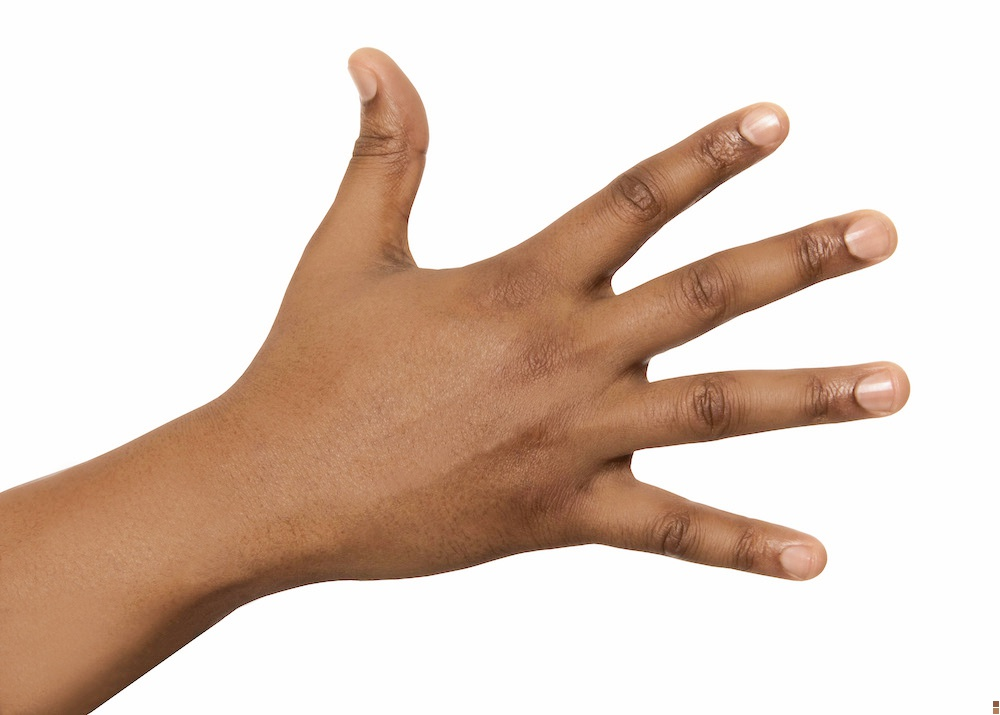
\includegraphics[width=\textwidth,height=\textheight,keepaspectratio]{../rc_test/outputs/20170524_prop_corr_1p1_ave_5/hand_dark_to_hand_brown.jpg}
  \end{minipage} \\
\hline
	  \label{row:PY_NAME_hand_dark_to_hand_light} &
  \begin{minipage}{.29\textwidth}
    \includegraphics[width=\textwidth,height=\textheight,keepaspectratio]{../inputs/hand_dark.jpg}
  \end{minipage} & 
  \begin{minipage}{.29\textwidth}
    \includegraphics[width=\textwidth,height=\textheight,keepaspectratio]{../inputs/hand_light.jpg}
  \end{minipage} & 
  \begin{minipage}{.29\textwidth}
    \includegraphics[width=\textwidth,height=\textheight,keepaspectratio]{../rc_test/outputs/20170524_prop_corr_1p1_ave_5/hand_dark_to_hand_light.jpg}
  \end{minipage} \\
\hline
	  \label{row:PY_NAME_hand_dark_to_hand_pale} &
  \begin{minipage}{.29\textwidth}
    \includegraphics[width=\textwidth,height=\textheight,keepaspectratio]{../inputs/hand_dark.jpg}
  \end{minipage} & 
  \begin{minipage}{.29\textwidth}
    \includegraphics[width=\textwidth,height=\textheight,keepaspectratio]{../inputs/hand_pale.jpg}
  \end{minipage} & 
  \begin{minipage}{.29\textwidth}
    \includegraphics[width=\textwidth,height=\textheight,keepaspectratio]{../rc_test/outputs/20170524_prop_corr_1p1_ave_5/hand_dark_to_hand_pale.jpg}
  \end{minipage} \\
\hline
	  \label{row:PY_NAME_hand_brown_to_hand_dark} &
  \begin{minipage}{.29\textwidth}
    \includegraphics[width=\textwidth,height=\textheight,keepaspectratio]{../inputs/hand_brown.jpg}
  \end{minipage} & 
  \begin{minipage}{.29\textwidth}
    \includegraphics[width=\textwidth,height=\textheight,keepaspectratio]{../inputs/hand_dark.jpg}
  \end{minipage} & 
  \begin{minipage}{.29\textwidth}
    \includegraphics[width=\textwidth,height=\textheight,keepaspectratio]{../rc_test/outputs/20170524_prop_corr_1p1_ave_10/hand_brown_to_hand_dark.jpg}
  \end{minipage} \\
\hline
	  \label{row:PY_NAME_hand_brown_to_hand_light} &
  \begin{minipage}{.29\textwidth}
    \includegraphics[width=\textwidth,height=\textheight,keepaspectratio]{../inputs/hand_brown.jpg}
  \end{minipage} & 
  \begin{minipage}{.29\textwidth}
    \includegraphics[width=\textwidth,height=\textheight,keepaspectratio]{../inputs/hand_light.jpg}
  \end{minipage} & 
  \begin{minipage}{.29\textwidth}
    \includegraphics[width=\textwidth,height=\textheight,keepaspectratio]{../rc_test/outputs/20170524_prop_corr_1p1_ave_100/hand_brown_to_hand_light.jpg}
  \end{minipage} \\
\hline
	  \ref{row:PY_NAME_hand_brown_to_hand_pale} &
  \begin{minipage}{.29\textwidth}
    \includegraphics[width=\textwidth,height=\textheight,keepaspectratio]{../inputs/hand_brown.jpg}
  \end{minipage} & 
  \begin{minipage}{.29\textwidth}
    \includegraphics[width=\textwidth,height=\textheight,keepaspectratio]{../inputs/hand_pale.jpg}
  \end{minipage} & 
  \begin{minipage}{.29\textwidth}
    \includegraphics[width=\textwidth,height=\textheight,keepaspectratio]{../rc_test/outputs/20170524_prop_corr_1p1_ave_25/hand_brown_to_hand_pale.jpg}
  \end{minipage} \\
\hline
	  \label{row:PY_NAME_hand_light_to_hand_dark} &
  \begin{minipage}{.29\textwidth}
    \includegraphics[width=\textwidth,height=\textheight,keepaspectratio]{../inputs/hand_light.jpg}
  \end{minipage} & 
  \begin{minipage}{.29\textwidth}
    \includegraphics[width=\textwidth,height=\textheight,keepaspectratio]{../inputs/hand_dark.jpg}
  \end{minipage} & 
  \begin{minipage}{.29\textwidth}
    \includegraphics[width=\textwidth,height=\textheight,keepaspectratio]{../rc_test/outputs/20170524_prop_corr_1p1_ave_5/hand_light_to_hand_dark.jpg}
  \end{minipage} \\
\hline
	  \label{row:PY_NAME_hand_light_to_hand_brown} &
  \begin{minipage}{.29\textwidth}
    \includegraphics[width=\textwidth,height=\textheight,keepaspectratio]{../inputs/hand_light.jpg}
  \end{minipage} & 
  \begin{minipage}{.29\textwidth}
    \includegraphics[width=\textwidth,height=\textheight,keepaspectratio]{../inputs/hand_brown.jpg}
  \end{minipage} & 
  \begin{minipage}{.29\textwidth}
    \includegraphics[width=\textwidth,height=\textheight,keepaspectratio]{../rc_test/outputs/20170524_prop_corr_1p1_ave_5/hand_light_to_hand_brown.jpg}
  \end{minipage} \\
\hline
	  \label{row:PY_NAME_hand_light_to_hand_pale} &
  \begin{minipage}{.29\textwidth}
    \includegraphics[width=\textwidth,height=\textheight,keepaspectratio]{../inputs/hand_light.jpg}
  \end{minipage} & 
  \begin{minipage}{.29\textwidth}
    \includegraphics[width=\textwidth,height=\textheight,keepaspectratio]{../inputs/hand_pale.jpg}
  \end{minipage} & 
  \begin{minipage}{.29\textwidth}
    \includegraphics[width=\textwidth,height=\textheight,keepaspectratio]{../rc_test/outputs/20170524_prop_corr_1p1_ave_25/hand_light_to_hand_pale.jpg}
  \end{minipage} \\
\hline
	  \ref{row:PY_NAME_hand_pale_to_hand_dark} &
  \begin{minipage}{.29\textwidth}
    \includegraphics[width=\textwidth,height=\textheight,keepaspectratio]{../inputs/hand_pale.jpg}
  \end{minipage} & 
  \begin{minipage}{.29\textwidth}
    \includegraphics[width=\textwidth,height=\textheight,keepaspectratio]{../inputs/hand_dark.jpg}
  \end{minipage} & 
  \begin{minipage}{.29\textwidth}
    \includegraphics[width=\textwidth,height=\textheight,keepaspectratio]{../rc_test/outputs/20170524_prop_corr_1p1_ave_5/hand_pale_to_hand_dark.jpg}
  \end{minipage} \\
\hline
	  \ref{row:PY_NAME_hand_pale_to_hand_brown} &
  \begin{minipage}{.29\textwidth}
    \includegraphics[width=\textwidth,height=\textheight,keepaspectratio]{../inputs/hand_pale.jpg}
  \end{minipage} & 
  \begin{minipage}{.29\textwidth}
    \includegraphics[width=\textwidth,height=\textheight,keepaspectratio]{../inputs/hand_brown.jpg}
  \end{minipage} & 
  \begin{minipage}{.29\textwidth}
    \includegraphics[width=\textwidth,height=\textheight,keepaspectratio]{../rc_test/outputs/20170524_prop_corr_1p1_ave_100/hand_pale_to_hand_brown.jpg}
  \end{minipage} \\
\hline
	  \ref{row:PY_NAME_hand_pale_to_hand_light} &
  \begin{minipage}{.29\textwidth}
    \includegraphics[width=\textwidth,height=\textheight,keepaspectratio]{../inputs/hand_pale.jpg}
  \end{minipage} & 
  \begin{minipage}{.29\textwidth}
    \includegraphics[width=\textwidth,height=\textheight,keepaspectratio]{../inputs/hand_light.jpg}
  \end{minipage} & 
  \begin{minipage}{.29\textwidth}
    \includegraphics[width=\textwidth,height=\textheight,keepaspectratio]{../rc_test/outputs/20170524_prop_corr_1p1_ave_100/hand_pale_to_hand_light.jpg}
  \end{minipage} \\
\hline

 \end{longtable}

Figure \ref{img:10_perc_mask} demonstrates the new regions used to calculate the average skin colour. We can see that the areas with shadows are effectively discarded, and the average colour calculated is significantly lighter and visually more accurate to the skin colour of the target hand. 

\begin{figure}[H]
\centering
\begin{tabular}{ccc}
    \multirow{2}{*}[5em]{\begin{subfigure}[b]{0.30\textwidth}
        \includegraphics[width=\textwidth]{images/hand_pale}
        \caption{Input hand image with significant shadows}\label{img:alg_3_eval_hand_pale}
    \end{subfigure}}&
    \begin{subfigure}[b]{0.30\textwidth}
        \includegraphics[width=\textwidth]{images/pale_ave_10_original_mask}
        \caption{Mask used to calculate color in Algorithm \ref{eq:prop_corr_algo}}\label{img:original_mask}
    \end{subfigure} &
    \begin{subfigure}[b]{0.30\textwidth}
        \includegraphics[width=\textwidth]{images/ave_col_100}
        \caption{Average color calculated with Algorithm \ref{eq:prop_corr_algo}}\label{img:ave_col_100}
    \end{subfigure}\\
    &
    \begin{subfigure}[b]{0.30\textwidth}
        \includegraphics[width=\textwidth]{images/pale_ave_10_adjusted_mask}
        \caption{Mask used to calculate color in Algorithm \ref{eq:prop_corr_ave_algo}}\label{img:adjusted_mask}
    \end{subfigure} &
    \begin{subfigure}[b]{0.30\textwidth}
        \includegraphics[width=\textwidth]{images/ave_col_10}
        \caption{Average color calculated with Algorithm \ref{eq:prop_corr_ave_algo}}\label{img:ave_col_10}
    \end{subfigure}
\end{tabular}
\caption{The average color calculation process in Algorithm \ref{eq:prop_corr_ave_algo} compared to that in the previous version, Algorithm \ref{eq:prop_corr_algo}}\label{img:10_perc_mask}
\end{figure}

As a result of the more accurate target colour, the resulting output image is more accurate to the colour of the hand in the target image, as show in Figure \ref{img:compare_perc}

\begin{figure}[H]
    \centering
    \begin{subfigure}[b]{0.40\textwidth}
        \includegraphics[width=\textwidth]{../rc_test/outputs/20170522_proportional_corrected_test_alpha1p1/hand_light_to_hand_pale.jpg}
        \caption{Output obtained using all pixels for target average (Algorithm \ref{eq:prop_corr_algo})}
    \end{subfigure}
    ~
    \begin{subfigure}[b]{0.40\textwidth}
        \includegraphics[width=\textwidth]{../rc_test/outputs/20170524_prop_corr_1p1_ave_10/hand_light_to_hand_pale.jpg}
        \caption{Output obtained using brightest pixels for target average (Algorithm \ref{eq:prop_corr_ave_algo})}
    \end{subfigure}
    \caption{Comparison of Algorithms \ref{eq:prop_corr_algo} and \ref{eq:prop_corr_ave_algo} results for transforming a light hand (Figure \ref{img:input_hands_1_light}) to a pale hand (Figure \ref{img:input_hands_1_pale}).\label{img:compare_perc}}
\end{figure}

We note that, overall, the more moderate skin colour changes which use mid-toned and light hands as the source image in Rows \ref{row:prop_corr_ave_test_hand_brown_to_hand_dark} to \ref{row:prop_corr_ave_test_hand_light_to_hand_pale} now show relatively realistic and accurate results. However, for other tests with more extreme colour changes, such as in Row \ref{row:prop_corr_ave_test_hand_dark_to_hand_pale} and \ref{row:prop_corr_ave_test_hand_pale_to_hand_dark}, the colour change is still not convincing.
